\documentclass[12pt]{article}

\usepackage{sbc-template}

\usepackage{graphicx,url}

%\usepackage[brazil]{babel}
\usepackage[utf8]{inputenc}

\usepackage{amsmath}
\usepackage{listings}
\usepackage{xspace}

%% workaround hyperref was messing with bib
%https://tex.stackexchange.com/a/125568/208799
\makeatletter
\newcommand{\@BIBLABEL}{\@emptybiblabel}
\newcommand{\@emptybiblabel}[1]{}
\makeatother
\usepackage{hyperref}% Enables \autoref
%%%%%%%%%

\usepackage{tabularx}
\usepackage[table]{xcolor}
\usepackage{caption}
\usepackage{subcaption}
\usepackage{bold-extra}
% \setlength\extrarowheight{2pt} % make the tables look less cramped

\usepackage{tikz}
\usetikzlibrary{shapes.misc, shapes.symbols, fit, positioning, quotes}

\usepackage[inline]{enumitem} % inline lists


\usepackage{tcolorbox}
\usepackage{soul}
\sethlcolor{red}
\newcommand{\mycommentbox}[1]{%
  \begin{tcolorbox}[colback=red!20!white,colframe=red,title=Comment]
      #1
  \end{tcolorbox}
}
\newcommand{\mycomment}[1]{%
	\hl{#1}
}

\newlist{inlinelist}{enumerate*}{1}
\setlist[inlinelist]{label=(\roman*)}



\newcommand{\pathsec}{\textbf{PathSec}\xspace}
\newcommand{\nodeid}{\texttt{node\_id}\xspace}
\newcommand{\nodeids}{\texttt{node\_id}s\xspace}
\newcommand{\portid}{\texttt{port\_id}\xspace}
\newcommand{\portids}{\texttt{port\_id}s\xspace}
\newcommand{\routeid}{\texttt{route\_id}\xspace}
\newcommand{\routeids}{\texttt{route\_id}s\xspace}
\newcommand{\timestamp}{\texttt{timestamp}\xspace}
\newcommand{\lhash}{\texttt{l\_hash}\xspace}
\newcommand{\nhop}{\texttt{nhop}\xspace}
\newcommand{\polka}{\textit{PolKA}\xspace}
\newcommand{\pIV}{\textit{P4}\xspace}
\newcommand{\bmv}{\textit{BMv2}\xspace}
\newcommand{\siphash}{\textit{Siphash}\xspace}


\sloppy

\title{Implementing and Testing a Probing-Based Path Verification for PolKA Source Routing Protocol}

\author{Henrique C. Layber, Roberta L. Gomes, Magnos Martinello}


\address{Department of Informatics\\Federal University of Espírito Santo (UFES) -- Vitória, ES -- Brazil
\email{henrique.layber@edu.ufes.br,\{roberta.gomes, magnos.martinello\}@ufes.br}
}



\begin{document} 

\maketitle

\begin{abstract}
    This work presents an implementation as proof-of-concept  for testing of a path-aware routing named \pathsec. It relies on a path probing and verification mechanism for the source-routing protocol \polka. The mechanism leverages a combination of hash functions, computed by stateless core switches, enabling a trusted party to verify whether a packet traversed the network along the source-defined path. The implementation was carried out in Mininet using BMv2 switches programmed in P4. Different adversity scenarios are evaluated to assess the system's robustness and security against specific attacks. The results confirm that the probing-based approach successfully detected the various path deviation attacks or misconfigurations.

    
\end{abstract}
     
\begin{resumo} 
    %Este trabalho apresenta uma implementação como prova-de-conceito para testes do \pathsec\cite{pathsec}, um mecanismo de sondagem e verificação de rota para o protocolo de roteamento na origem \polka. O mecanismo é baseado em uma combinação de funções hash, calculadas por switches de núcleo sem estado, e permitem uma parte confiável verificar se um pacote percorreu a rede ao longo do caminho definido pela origem. A implementação foi feita no Mininet usando BMv2 programados em P4.
Este trabalho apresenta uma implementação como prova de conceito para testar um roteamento ciente de caminho denominado \pathsec. O trabalho se baseia em um mecanismo de sondagem e verificação de caminho para o protocolo de roteamento de fonte \polka. O mecanismo utiliza uma combinação de funções hash, calculadas por switches de núcleo sem estado, permitindo que uma entidade confiável verifique se um pacote percorreu a rede conforme o caminho definido na origem. A implementação foi realizada no Mininet usando switches BMv2 programados em P4. Diferentes cenários adversos foram avaliados para testar a robustez e segurança do sistema contra ataques específicos. Os resultados confirmam que a abordagem baseada em sondagem detectou com sucesso diversos ataques de desvio de caminho ou configurações incorretas.
\end{resumo}

{\footnotesize\textbf{Keywords -- Path Aware; Network Security; Path Verification; In-networking Programming}}


% Probing
\section{Introduction}
% O que foi feito
% Motivaçao (!!)
% Oq é SR e Probe-Based Verification (PBV)

% - motivação source routing
% - com isso, há a proposta do polka (sistema de resíduos sem explicar o que é precisamente)
% - mas que que há uma limitação: como comprovar que de fato a rota foi respeitada
% - foi criada a solução do pathsec
% ...
% - contexto deste trabalho: a implementação e testes do pathsec no mininet

Ever since \textit{Source Routing} (SR) was proposed, there has been a need to ensure that packets traverse the network along the paths selected by the source, not only for security reasons, but also to ensure that the network is functioning 
%BETA
%correctly
properly
and correctly configured. This is particularly important in the context of \textit{Software-Defined Networks} (SDNs), where the control plane can select paths based on a variety of criteria\cite{SRSDN}.

In this paper, we propose an implementation on Programming Protocol Independent Processors (\pIV) for 
%BETA
%Probing-Based Path Verification (PBV),
a Probing-Based Path Verification (PBV) mechanism originally proposed in \pathsec\cite{pathsec}. 
This mechanism provides proofs of packet forwarding (\textit{proof-of-transit}), confirming that an expected route was indeed used for a packet.
This is achieved by using a composition of hash functions on stateless core switches, 
%BETA
combined with the switches native secret code (\nodeids) and the respective route's output port, which results into a lightweight multi-signature. 


In the complete solution proposed by \pathsec, once packets reach the egress edges, the final lightweight multi-signatures are extracted from the packets and sent to smart contracts deployed in a blockchain. These signatures are then compared to reference signatures previously registered by a trusted party (the network controller), allowing to verify packets' \textit{proof-of-transit} and to register path compliance. Blockchain, smart contracts and signature checking in deployment conditions is out of scope for this work. For this work, the scope is to generate the signatures for packets and verify how the system behaves.



% This signature  can then be compared
% %BETA
% to a reference signature generated by a trusted party, the network controller.
% %BETA
% %This work tests a proof-of-concept implementation under different adversity scenarios and results show the approach is effective as a proof-of-transit solution.




The proof-of-concept implementation was then tested under different adversity scenarios, and the results show that the approach is effective as a proof-of-transit solution. All the code and test results are available online\footnote{\url{github.com/Henriquelay/pathsec-poc}}. 
This work extends previous work that implements \polka in Mininet\cite{polkap4}\footnote{\url{github.com/nerds-ufes/polka}}, by adding support to \pathsec.




The structure of this paper is as follows: \autoref{sec:definition} outlines the problem definition and the proposed solution; \autoref{sec:implementation} describes the implementation details, including the architecture and the employed tools; \autoref{sec:testing} presents the scenarios used to evaluate the system and the results, and \autoref{sec:conclusion} concludes the paper.


\section{Problem definition} \label{sec:definition} 

% Top to bottom, indo do sistema mais amplo ao programa em baixo nível


The \pathsec approach for proof-of-transit uses a logically centralized SDN Controller that selects routing paths and configures the core and edge nodes. While ingress and egress edges encapsulates/decapsulates metadata into/from packets, core nodes execute hashing operations alongside basic \polka packet forwarding.

%Calculating each hop is done exploiting the Chinese Remainder Theorem\cite{polka}, and is out of the scope of this paper. 
\pathsec is based on \polka's source routing which explores the Chinese Remainder Theorem\cite{polka}.
\polka assigns a unique route identifier (\routeid) to each path in the core network, and for each core switch it defines a unique \nodeid. Once a packet is associated to a specific route, each packet in this packet  will carry in its header the respective \routeid (embeded by the ingress edge). Then the core switches use the \routeid field and their respective \nodeids to calculate the output \portid (it is a result of the Residue Number System (RNS)-based encoding\cite{pathsec}, which is out of the scope of this paper), routing the packets to the next core node in the expected path for the \routeid.

Furthermore, \pathsec designs a simplified signing mechanism using the uniqueness of the switch-port pair (\nodeid, \portid) for each \routeid, and by holding these components in as a secret, they can be used together as keys for cryptographic hashing functions. Every switch-port pair acts as a native secret information by not being shared in the resulting message, enabling a lightweight multi-signature scheme based on Hash-based Message Authentication Code (HMAC): before routing a packet, a core node replaces the lightweight signature from the previous core node (embedded in the packet header), with a new one, hashing the previous one with the pair (\nodeid, \portid). This mechanism ensures an inherent property of the routing system that facilitates efficient path verification. 

%BETA: JOGUEI PARA A SUBSEC ANTERIOR (INTRODUÇÃO)
%In the complete solution proposed by \pathsec, once packets reach the egress edges, the final lightweight multi-signatures are extracted from the packets and sent to smart contracts deployed in a blockchain. These signatures are then compared to reference signatures previously registered by a trusted party (the network controller), allowing to verify packets' \textit{proof-of-transit} and to register path compliance. Blockchain, smart contracts and signature checking in deployment conditions is out of scope for this work. For this work, the scope is to generate the signatures for packets and verify how the system behaves.


% \anotacao{Acho que esse título (ou conteúdo) pode melhorar. O \pathsec não diz explícitamente que usar o \polka, então parece "irrelevante" pro propósito do artigo}


\subsection{Problem formalization} \label{sec:formalization}
\newcommand{\Pie}{P_{i \rightarrow e}}

Let $i$ be the source node (\textbf{i}ngress node) and $e$ be the destination node (\textbf{e}gress node). Let the path from $i$ to $e$ $\Pie$ be a sequence of nodes: the path is defined by $ \Pie = (i, s_1, s_2, ..., s_{n - 1}, s_n, e) $\label{eq:path-def}, $s_n$ being the $n$-th core node in the path. In SR protocols, packets' routes through the core network are defined in $i$. That is, $i$ sets the packet header with enough information for each core node to calculate the next hop. 


The main problem we are trying to solve is path verification, that is, to have a way to ensure if the packet follows the path defined. A solution must be able to identify if the packet:
\begin{inlinelist}
    \item has passed through all nodes in the Path;
    \item has passed through the correct order of nodes;
    \item has \textbf{not} passed through any node that is \textbf{not} in the path.
\end{inlinelist}




More formally, given a routed sequence of nodes $P_{i \rightarrow e}$, and a captured sequence of nodes actually traversed $P_j$, a solution must identify if $P_{i \rightarrow e} = P_j$.
Notably, it does not require validation, that is, it needs only to respond if $P_{i \rightarrow e} = P_j$ and does not need to know any of their contents or check their validity as a route.


\subsection{Multi-signature model for Path Verification} \label{sec:multisigmodel}
%cite pathsec

To balance trace effectiveness and scalability, \pathsec proposes using packets themselves as probes\cite{pathsec}\cite{PINT2020}, with a lightweight multi-signature, keeping the header size fixed. That is, each core node hashes the previous node's signature with a key only itself (and the Controller) can possess, and pass the hash result forward, replacing the previous hash results, and all following core nodes will do the same until the edge node is reached. There is a cost to this write operation, especially when analyzing relative to \polka since \polka does not require any part of the packet to be written on in the whole route, but since header size is fixed, and not all packets are expected to contain probing metadata, the cost is mitigated.

Each node's execution plan is stateless. So, in terms of signature composition, a node $n_i$ can be viewed as a function $f_{n_i} (x)$. A node can alter the header of the packet, which
%BETA
% we will use
is used to push information downstream,
%and 
allowing ultimately to detect if the path taken is correct.
%BETA
%\mycomment{Está preciso e claro dizer que ``which we will use to push information downstream''?}

In order to represent all nodes by the same function, we assign a distinct key value $k_{n}$ for each node $n$, and use a bivariate function $f(k_{n}, x) = f_{n} (x)$.
By using functions in two variables and enforcing one of the variables assume a value that's unique between nodes, we ensure that the function's result is unique for each switch as long as the function is collision resistant enough, that is, $f_{a} (x) \neq f_{b} (x) \iff a \neq b$.

Using function composition is appropriate, as it preserves the order-sensitive property of the path, since $f \circ g \neq g \circ f$ in a general case.
In our model, each node will execute a single function of this composition, using the previous node's output as input.
In this way, $ (f_{n_1} \circ f_{n_2} \circ f_{n_3})(x) = f(k_{n_3}, f(k_{n_2}, f(k_{n_1}, x))) $, $f$ being a function sufficiently resistant to collision. A cryptographic hash function is essential for maintaining the security of sensitive data. A strong avalanche effect is particularly desirable, ensuring that even minor variations in the input produce significantly different hash values. While the computational cost of cryptographic hash functions is higher compared to non-cryptographic alternatives, modern algorithms such as BLAKE2\cite{BLAKE2} and SipHash\cite{siphash} have significantly reduced this performance gap, making them viable choices for both security and efficiency.

\tikzset{
  host/.style={
    scale=\nodescale,
    inner sep=1pt,
    draw,
    rounded rectangle,
  },
  edge/.style={
    scale=\nodescale,
    inner sep=1pt,
    draw,
    rounded rectangle,
    fill=blue!20,
  },
  core/.style={
    scale=\nodescale,
    inner sep=1pt,
    draw,
    rounded rectangle,
    fill=green!30,
  },
  port/.style = {
    % font=\tiny,
    scale=.5,
    inner sep=1pt,
    draw,
    signal,
    fill=white,
  }
}
\newcounter{previtem}

\section{Implementing and Testing a Probing-Based Path Verification (PBV)} \label{sec:implementation}

PBV consists of sending special packets (probes) with path-verification capabilities. The path verification system used is described in \autoref{sec:multisigmodel}. Some assumptions are made:
\begin{inlinelist}
    \item Each node is assumed to be secure, that is, no node will alter the packet in any way that is not expected. This is a common assumption in SDN networks, where a trusted party is the only entity that can alter the network state;
    \item  Every link is assumed to be perfect, that is, no packet loss, no packet corruption, and no packet duplication;
    \item  Protocol boundary is IPv4, this means that 
    %BETA
    %\polka
    \pathsec is only used inside this network, and only IPv4 is used outside; \label{assumption:ipv4}
    \item All paths are assumed to be valid and all information correct unless stated otherwise.
\end{inlinelist}
Furthermore, this implementation is a proof-of-concept, and there is little concerns about performance other protocol support. The tests were made using an ICMP (ping) packet. The following subsections detail the setup and implementation.

\subsection{Setup}

\pIV is a language used to program the data plane of network devices \cite{p4}. Behavioral Model 2 (\bmv) is a software switch that supports the \pIV language \cite{bmv2}. Mininet is a network emulation tool that allows the creation of virtual networks with a controlled environment \cite{mininet}. Mininet-wifi\cite{mininet-wifi} is a Mininet fork used in this work due to its compatibility with \bmv. Despite the name, no Wi-Fi emulating feature was used.

The Controller is responsible for the network setup and for calculating reference signatures.
In our implementation, the Python Script that controls Mininet acts a controller, and itself is not a network entity in Mininet.
Scapy is a Python library that allows the creation and manipulation of packets \cite{scapy}. It is used to sniff packets both for Controller operation and in the experiments and automate tests. 
The Tester is responsible for triggering Mininet hosts to send packets, setting up Scapy for parsing them and then asserting their signatures to Controller-calculated references. Only Scapy's sniffing capabilities were used, and tests were performed with a regular \texttt{ICMP} packet (\textit{ping}).
The setup is shown in \autoref{setup}. 


\subsection{Implementation}

We define the header fields \timestamp and \lhash, both 32-bits wide, to indicate the uniquely-generated number and the current lightweight multi-signature, respectively.

To maintain \polka protocol compatibility, probe packets are identified by a different version number in \polka's \texttt{version} field, so interoperates with \polka depending on the \texttt{version} header. Regular \polka packets use version \texttt{0x01}, and probe packets (with \timestamp and \lhash fields) use version \texttt{0xF1}.

\autoref{topology:base} shows the used topology used in the experiments where $s_i$ is a switch, $e_i$ is an edge node, and $h_i$ is a host. The topology is a linear chain with 10 switches and 11 hosts. The links are bidirectional, but only one direction is shown for simplicity. %The ports are numbered from $1$ to $3$, and the ports used are shown in the figure. The topology is used to test the path verification mechanism.

\begin{figure}[ht]
    \centering
    \begin{subfigure}[b]{0.49\linewidth}
    \centering
    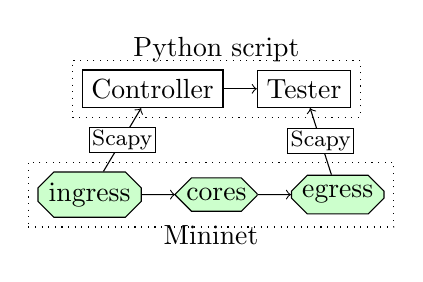
\begin{tikzpicture}[
        outer sep=auto,
        every node/.style={draw, rectangle, label distance=-4pt},
        switch/.style={chamfered rectangle, fill=green!20, inner sep=1pt},
        % every fit/.style={rectangle,draw}
    ]
        \node (controller) {Controller};
        \node[right=12pt of controller] (tester) {Tester};
        \draw[->] (controller) to (tester);
        \node[label=above:Python script, dotted,
          fit={(controller) (tester)}] (py) {};

        \node[switch, below=32pt] at (py) (s1) {cores};
        \node[switch, left=12pt] at (s1.west) (ingress) {ingress};
        \node[switch, right=12pt] at (s1.east)      (egress) {egress};
        \draw[->] (ingress) to (s1);
        \draw[->] (s1) to (egress);
        \node[label=below:Mininet, dotted,
            fit={(ingress) (s1) (egress)}] {};

        \draw[->] (ingress) -- node[fill=white, inner sep=1pt] {\footnotesize Scapy} (controller);
        \draw[->] (egress) -- node[fill=white, inner sep=1pt] {\footnotesize Scapy} (tester) ;
    \end{tikzpicture}
    \caption{Experimentation setup.\\Arrows show data flow.}
    \label{setup}
    \end{subfigure}
    \hfill
    \begin{subfigure}[b]{0.49\linewidth}
    \centering    
    \newcommand{\nodescale}{0.8}
    \newcommand{\nswitches}{10}
    \newcommand{\newtopoitem}[2]{%
        \node[host, right=2pt] (H#1) at (H#2.east)  {$h_{#1}$};
        \node[edge, above=4pt] (E#1) at (H#1.north) {$e_{#1}$};
        \node[core, above=4pt] (S#1) at (E#1.north) {$s_{#1}$};
        \draw (H#1) -- (E#1) -- (S#1);
    }
    \setcounter{previtem}{11}
    \begin{tikzpicture}[outer sep=auto]
        \node[host] (H11) {$h_{11}$};
        \foreach \x in {1, ..., \nswitches} {
            \newtopoitem{\x}{\arabic{previtem}}
            \ifnum \theprevitem < 11
                \draw (S\x) to (S\theprevitem);
            \fi
            \setcounter{previtem}{\x}
        }
        \draw (H11) to (E1);
            
    \end{tikzpicture}
    \caption{Baseline topology used in experimentation.}
    \label{topology:base}
    \end{subfigure}
    \hfill
      \vspace{0.5cm}
% \end{figure}
% Joins both figures into one
% \begin{figure}[ht]
%     \centering
    \tikzset{
        outer sep=auto,
        every node/.style={draw, chamfered rectangle, label distance=-4pt, inner sep=2pt},
    }
    \begin{subfigure}[b]{0.49\linewidth}
    \centering    
    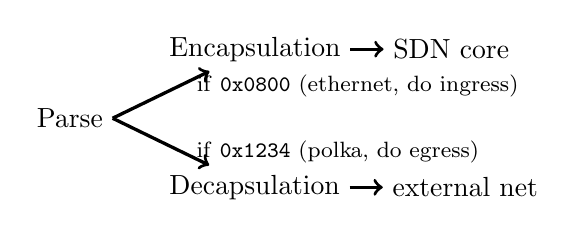
\begin{tikzpicture}
        \node (parse) {Parse};
            
        \node[above right=24pt] (encap) at (parse.east) {Encapsulation};
        \node[right=12pt] (core) at (encap.east) {SDN core};
        \draw[->, very thick] (parse.east) -- (encap)
            node[draw=none,pos=0.7,xshift=2pt,anchor=mid west] {\footnotesize if \texttt{0x0800} (ethernet, do ingress)};
        \draw[->, very thick] (encap) -- (core);
        
        \node[below right=24pt] (decap) at (parse.east) {Decapsulation};
        \node[right=12pt] (out) at (decap.east) {external net};
        \draw[->, very thick] (parse.east) -- (decap)
            node[draw=none,pos=0.7,xshift=2pt, anchor=mid west] {\footnotesize if \texttt{0x1234} (polka, do egress)};
        \draw[->, very thick] (decap) -- (out);
    \end{tikzpicture}
    \caption{Edge ingress/egress pipeline.}
    \label{fig:pipeline-edge}
    \end{subfigure}
    \hfill
    \begin{subfigure}[b]{0.49\linewidth}
    \centering    
    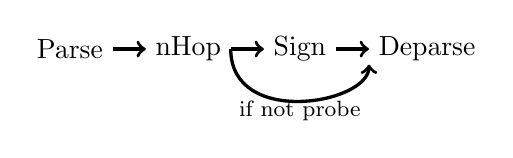
\begin{tikzpicture}
        \node (parse) {Parse};
        \node[right=12pt] (nhop) at (parse.east) {nHop};
        \node[right=12pt] (sign) at (nhop.east) {Sign};
        \node[right=12pt] (deparse) at (sign.east) {Deparse};

        \draw[->, very thick] (parse) -- (nhop);
        \draw[->, very thick] (nhop) -- (sign);
        \draw[->, very thick] 
            (nhop.east) ..controls ++(0,-1) and ++(0,-0.5) .. (deparse.195) node[midway,below=-4pt,draw=none] {\footnotesize if not probe};
        \draw[->, very thick] (sign) -- (deparse);
            
    \end{tikzpicture}
    \caption{Data plane core pipeline.}
    \label{fig:pipeline-core}
    \end{subfigure}
    \caption{Implementation description.}
    \label{fig:implementation}
\end{figure}

Edge nodes can receive both \polka packets or IPv4 packets. If the IPv4 protocol \texttt{ethertype} header field is detected (\texttt{0x0800}), it must be a packet from outside the network, so it proceeds with the role of an ingress edge and \polka headers need to be added. Let this process be called \textit{encapsulation}. If a \polka protocol \texttt{ethertype} field is detected (\texttt{0x1234}), it must be a packet from the network core, so it proceeds with the role of an egress edge and the original IPv4 packet must be unwrapped. Let this process be called \textit{decapsulation}. This flow is illustrated in \autoref{fig:pipeline-edge}.

\polka headers consists of the route polynomial (\routeid), along with \texttt{version}, \texttt{ttl} and \texttt{proto} (stores the original \texttt{ethertype}).
% \routeid and hop calculation is out of the scope of this paper.
During encapsulation, the packet can be made into a probe packet by setting the \texttt{version} header field to \texttt{0xF1} and further defining the 32-bit fields \timestamp to any unique value and \lhash initially equal to \timestamp.

On the core network, illustrated on \autoref{fig:pipeline-core}, the hash function used in the \textit{Sign} step is \textit{SipHash-2-4-32}\cite{siphash} (\siphash). It is expected to provide maximum MAC security possible for $c \geq 2$ and $d \geq 4$. The function is not made to be collision-resistant, but its features are well-suited to be used as a MAC\cite{siphash}. 
Hash collisions for a small scale test like we present is extremely unlikely, since our hash output is evaluated to be indistinguishable from a uniform random function, and collisions would need to happen in the same route for impacts to occur.
%BETA
%which 
After calculating the next output port (\nhop) and if the packet is a probe packet, \lhash is computed as
$$
\lhash \leftarrow \textit{SipHash2-4-32}(\nodeid || \nhop || \timestamp || \texttt{0000000}, \lhash)
$$
Meaning that a 64-bit string made of concatenating \nodeid, \nhop, \timestamp with the remaining bits set to \texttt{0} for padding is used as key for the \siphash function hashing \lhash. 

\section{Testing} \label{sec:testing}

This section presents the results for various tests representing different adversity scenarios. Each scenario is designed to evaluate the robustness and security of the system under specific attack or misconfiguration conditions. 

\subsection{Adversity scenarios}\label{sec:adversity_scenarios}

The scenarios include addition, detour, skipping, and out-of-order packet delivery. We define any switch that is not in the position defined in \autoref{topology:base} as an \textit{attacker}, not only an intruder device, so it includes misconfigured switches, controller malfunction, and any other kind of network-affecting anomaly that results in these specified scenarios:

\begin{enumerate}[label=\roman*.]
    \item \label{scenario:addition} \textbf{Addition} (\autoref{topology:addition}): An attacker switch is added between $s_5$ and $s_6$. It perfectly replicates the behavior of the original switch, but it does not have the same \nodeid, as it is a secret key, and the hashes will not match when validating the path past the attacker.
    \item \label{scenario:skipping} \textbf{Skipping} (\autoref{topology:skipping}): A switch is removed between $s_4$ and $s_6$. The packet will skip removed switch, and the hashes will not match when validating the path past the removed switch.
    \item \label{scenario:detour} \textbf{Detour} (\autoref{topology:detour}): A switch is detoured between $s_5$ and $s_7$ into an attacker by hijacking the port that the packet should have taken exiting $s_5$ and delivering the packet in a new port to $s_7$, posing as $s_6$. The hashes will not match when validating the path past the attacker.
    \item \label{scenario:outoforder} \textbf{Out-of-order} (\autoref{topology:outoforder}): Links are changed between $s_5$ and $s_6$. The packet will be delivered to $s_6$ before $s_5$, and the hashes will not match when validating the path past the attack.
\end{enumerate}


\autoref{tab:adversity_checksums} shows the intermediary checksums for each scenario, highlighting the differences caused by the adversarial conditions, although in deployment, only the last \lhash ($s_{10}$) is every used for verification. Note that a scenario may result in a different amount of hashes to compare due to different amount of intermediary hops, so the table isn't completely filled to represent a hop that does not exist on a particular route. For all scenarios, a ping from $h_1$ to $h_{10}$ was performed, resulting in $\routeid = \texttt{0x707b3a1d61d1d0d8b9fc91e442d0360dfc8bba4}$.



\begin{figure}
    \centering
    \tikzset{
        host/.style={
            scale=\nodescale,
            inner sep=1pt,
            draw,
            rounded rectangle,
        },
        edge/.style={
            scale=\nodescale,
            inner sep=1pt,
            draw,
            rounded rectangle,
            fill=blue!20,
        },
        core/.style={
            scale=\nodescale,
            inner sep=1pt,
            draw,
            rounded rectangle,
            fill=green!30,
        },
        port/.style = {
            % font=\tiny,
            scale=.5,
            inner sep=1pt,
            draw,
            signal,
            fill=white,
        }
        }

    \newcommand{\nodescale}{0.8}
    \newcommand{\nswitches}{10}
    \newcommand{\newtopoitem}[2]{%
        \node[host, right=2pt] (H#1) at (H#2.east)  {$h_{#1}$};
        \node[edge, above=4pt] (E#1) at (H#1.north) {$e_{#1}$};
        \node[core, above=4pt] (S#1) at (E#1.north) {$s_{#1}$};
        \draw (H#1) -- (E#1) -- (S#1);
    }
    \newcommand{\newtopoitemanchors}[2]{%
        \node[core, below right=4pt] (S#1) at (#2.east)   {$s_{#1}$};
        \node[edge, below=4pt] (E#1) at (S#1.south) {$e_{#1}$};
        \node[host, below=4pt] (H#1) at (E#1.south) {$h_{#1}$};
        \draw (H#1) -- (E#1) -- (S#1);
    }
    \begin{subfigure}[t]{0.49\linewidth}
        \centering
        \newcommand{\splitpoint}{5} %switch is added after s5
        \setcounter{previtem}{11}
        \begin{tikzpicture}[outer sep=auto]
            \node[host] (H11) {$h_{11}$};
            \foreach \x in {1, ..., \splitpoint} {
                \newtopoitem{\x}{\arabic{previtem}}
                \ifnum \theprevitem < 11
                    \draw (S\x) to (S\theprevitem);
                \fi
                \setcounter{previtem}{\x}
            }
            \draw (H11) to (E1);

            \node[core, above right=4pt] at (S\theprevitem.east) (Sadd) {$s_{add}$};
            \newtopoitemanchors{6}{Sadd}
            \draw (S5) -- (Sadd) -- (S6);
            \stepcounter{previtem}

            \foreach \x in {\number\numexpr\splitpoint+2\relax, ..., \nswitches} {
                \newtopoitem{\x}{\arabic{previtem}}
                \draw (S\x) to (S\theprevitem);
                \setcounter{previtem}{\x}
            }
                
        \end{tikzpicture}
        \caption{Addition.}
        \label{topology:addition}
    \end{subfigure}
    \begin{subfigure}[t]{0.49\linewidth}
        \centering
        \newcommand{\splitpoint}{5} %switch is removed after s5
        \setcounter{previtem}{11}
        \begin{tikzpicture}[outer sep=auto]
            \node[host] (H11) {$h_{11}$};
            \foreach \x in {1,2,3,4,6,7,8,9,10} {
                \newtopoitem{\x}{\arabic{previtem}}
                \ifnum \theprevitem < 11
                    \draw (S\x) to (S\theprevitem);
                \fi
                \setcounter{previtem}{\x}
            }
            \draw (H11) to (E1);
                
        \end{tikzpicture}
        \caption{Skipping.}
        \label{topology:skipping}
    \end{subfigure}

    \begin{subfigure}{0.49\linewidth}
        \centering
        \newcommand{\splitpoint}{5} %switch is detoured after s5
        \setcounter{previtem}{11}
        \begin{tikzpicture}[outer sep=auto]
            \node[host] (H11) {$h_{11}$};
            \foreach \x in {1,...,\nswitches} {
                \newtopoitem{\x}{\arabic{previtem}}
                \ifnum \theprevitem < 11
                    \draw (S\x) to (S\theprevitem);
                \fi
                \setcounter{previtem}{\x}
            }
            \draw (H11) to (E1);

            \node[core, above=2pt, anchor=south] at (S6.north) (Sdet) {$s_{det}$};
            \draw (S5) -- (Sdet) -- (S7);
                
        \end{tikzpicture}
        \caption{Detour.}
        \label{topology:detour}
    \end{subfigure}
    \begin{subfigure}{0.49\linewidth}
        \centering
        \newcommand{\splitpoint}{5} %switch is changed after s5
        \setcounter{previtem}{11}
        \begin{tikzpicture}[outer sep=auto]
            \node[host] (H11) {$h_{11}$};
            \foreach \x in {1,2,3,4,6,5,7,8,9,10} {
                \newtopoitem{\x}{\arabic{previtem}}
                \ifnum \theprevitem < 11
                    \draw (S\x) to (S\theprevitem);
                \fi
                \setcounter{previtem}{\x}
            }
            \draw (H11) to (E1);                
        \end{tikzpicture}
        \caption{Out of order.}
        \label{topology:outoforder}
    \end{subfigure}

    \caption{Topologies for tested scenarios.}
    \label{fig:topologies}
\end{figure}

%attack model



\begin{table}
    \definecolor{Green}{HTML}{3C8031} % OliveGreen
    \newcommand{\red}[1]{\color{red}\texttt{\textbf{#1}}}
    \newcommand{\blu}[1]{\color{blue}\texttt{\textbf{#1}}}
    \newcommand{\grn}[1]{\color{Green}\texttt{\textbf{#1}}}
    \newcommand{\skp}{\cellcolor{black!30}}
    \newcommand{\headersize}{\small}
    \centering
    \scriptsize
    \begin{tabularx}{\linewidth}{ll|ll|ll|ll|ll}
        \hline
        \multicolumn{2}{c|}{\headersize Reference} & \multicolumn{2}{c|}{\headersize Addition} & \multicolumn{2}{c|}{\headersize Skipping} & \multicolumn{2}{c|}{\headersize Detour} & \multicolumn{2}{c}{\headersize Out-of-order} \\
         \hline%                        |          Add                   |       SKP                     |             DET                |         OOO
         \blu{$s_0$}   &\blu{0x61e8d6e7}&\grn{$s_0$}    &\grn{0x61e8d6e7}&\grn{$s_0$}   &\grn{0x61e8d6e7}&\grn{$s_0$}    &\grn{0x61e8d6e7}&\grn{$s_0$}    &\grn{0x61e8d6e7} \\ \hline
         \blu{$s_1$}   &\blu{0xd25dc935}&\grn{$s_1$}    &\grn{0xd25dc935}&\grn{$s_1$}   &\grn{0xd25dc935}&\grn{$s_1$}    &\grn{0xd25dc935}&\grn{$s_1$}    &\grn{0xd25dc935} \\ \hline
         \blu{$s_2$}   &\blu{0x245b7ac5}&\grn{$s_2$}    &\grn{0x245b7ac5}&\grn{$s_2$}   &\grn{0x245b7ac5}&\grn{$s_2$}    &\grn{0x245b7ac5}&\grn{$s_2$}    &\grn{0x245b7ac5} \\ \hline
         \blu{$s_3$}   &\blu{0xa3b38b83}&\grn{$s_3$}    &\grn{0xa3b38b83}&\grn{$s_3$}   &\grn{0xa3b38b83}&\grn{$s_3$}    &\grn{0xa3b38b83}&\grn{$s_3$}    &\grn{0xa3b38b83} \\ \hline
         \blu{$s_4$}   &\blu{0x26aee736}&\grn{$s_4$}    &\grn{0x26aee736}&\grn{$s_4$}   &\grn{0x26aee736}&\grn{$s_4$}    &\grn{0x26aee736}&\grn{$s_4$}    &\grn{0x26aee736} \\ \hline
         \blu{$s_5$}   &\blu{0xf9b47914}&\grn{$s_5$}    &\grn{0xf9b47914}&            &                  &\grn{$s_5$}    &\grn{0xf9b47914}&\red{$s_6$}    &\red{0x4b5a6c5a} \\ \hline
         \skp        &\skp              &\red{$s_{add}$}&\red{0x18c6d8d1}&\skp        &\skp              &\skp         &\skp              & \skp        &\skp               \\ \hline
         \blu{$s_6$}   &\blu{0x18c6d8d1}&\red{$s_6$}    &\red{0xb69b99ec}&\red{$s_6$}   &\red{0x4b5a6c5a}&\red{$s_{det}$}&\red{0x250822a2}&\red{$s_5$}    &\red{0xde3862a0} \\ \hline
         \blu{$s_7$}   &\blu{0xb69b99ec}&\red{$s_7$}    &\red{0xfe6117f8}&\red{$s_7$}   &\red{0x002346d3}&\red{$s_7$}    &\red{0x40298bb9}&\red{$s_7$}    &\red{0x648556ec} \\ \hline
         \blu{$s_8$}   &\blu{0xfe6117f8}&\red{$s_8$}    &\red{0xc8d9fbde}&\red{$s_8$}   &\red{0x7ec711aa}&\red{$s_8$}    &\red{0xe13dcc9b}&\red{$s_8$}    &\red{0x144e1d1b} \\ \hline
         \blu{$s_9$}   &\blu{0xc8d9fbde}&\red{$s_9$}    &\red{0xa6293a25}&\red{$s_9$}   &\red{0x5ee32b7b}&\red{$s_9$}    &\red{0x1bf62c19}&\red{$s_9$}    &\red{0x9e818f34} \\ \hline
         \blu{$s_{10}$}&\blu{0xa6293a25}&\red{$s_{10}$} &\red{0xf4bcdf07}&\red{$s_{10}$}&\red{0xc973a219}&\red{$s_{10}$} &\red{0xdd3a6675}&\red{$s_{10}$} &\red{0x06f694bc}  \\
         \hline
         \hline
    \end{tabularx}
    \caption{Intermediary \lhash for different test scenarios with the same seed.}
    \label{tab:adversity_checksums}
\end{table}

\subsection{Discussion}

Recovering data from Mininet switches is not trivial, as it does not provide a straightforward way to extract data from the switches. This limitation makes it difficult to analyze the data in real-time, so our solution depends on sniffer libraries (Scapy) to capture packets and extract the metadata. This limitation could be overcome by having the switches natively output the metadata to our controller, which would allow for a more performant and scalable solution. It was not implemented to keep the implementation minimal.

The cryptographically secure hash solution is only secure when the key is a secret. If the key is compromised, the entire system is compromised, as a malicious actor can easily generate the same checksums and be undetected, essentially signing whichever packets they want. Having the switch entry port included in the verification would mitigate this issue, as the attacker would need to know the exact port the packet entered the switch.

\section{Conclusion and Future Work} \label{sec:conclusion}


The implementation and evaluation of \pathsec demonstrate the feasibility of a path-aware routing mechanism that enhances network security through path verification. By leveraging hash-based authentication computed by stateless core switches, the system ensures that packets adhere to their intended routes, enabling a trusted entity to detect deviations caused by attacks or misconfigurations. The proof-of-concept implementation in Mininet with BMv2 switches programmed in \pIV highlights the practicality of deploying such a mechanism in programmable networks. The experimental results confirm the effectiveness of the probing-based approach in identifying various adversarial scenarios, reinforcing its potential as a security measure for source-routing protocols like \polka.  

While the study validates the fundamental principles behind \pathsec, future work could explore optimizations to improve scalability and efficiency in larger network deployments. Further research is needed to evaluate the system’s performance under high traffic loads and its adaptability to dynamic network conditions. Additionally, integrating \pathsec with other security mechanisms could enhance its resilience against more sophisticated attack strategies. Overall, this work provides a first step for advancing path-aware security in programmable networks and highlights the potential of verification-based approaches to strengthen network integrity.



%As the examples show, our solution is able to detect when a packet is not following the expected path for most cases, and can be used to detect misconfigurations in the network.

%As next steps, more parts of \pathsec \cite{pathsec} could be easily integrated for proof-of-concept, as all necessary information is already readily collect to Python scripts, making it simple to create 
%BETA
%a complete \pathsecproof-of-concept software.

%To improve the system for a real-world scenario, the ingress edge needs to relay the ingressed package metadata directly to the controller, and the egress edge will report the final checksum directly to the blockchain. Having it not passing through the controller.

%One type of attack is not detectable by the current solution, as the switch entry port is not included in the verification. Suppose a topology similar to our addition test (\autoref{scenario:addition}): $s_{add}$, as and attacker would receive the packet instead of $s_6$. $s_{add}$ can inspect or modify the packet as it wants, as long as \lhash field and \timestamp fields are untouched. As long as the verification headers are repeated when passing the packet forward to $s_6$, $s_6$'s hash will act upon the exact same inputs.

%Including the entry port in the checksum would also be an appreciable increase in security, since it increases the number of targets an attacker would need to breach at the same time to be able to alter the path. It could be included in the \siphash key, but a design decision is necessary: there are only 7 bits available, and the port number is 9 bits long. A possible solution would be to use the 8 least significant bits of the port number for both entry and exit port, limiting the number of ports checked before collision to 256, but this would be a reasonable trade-off for the increased security. It would mitigate attacks like previously described, where our probe headers are kept, and the remaining packet has changed. For a proof-of-concept, design was kept closer to the original \pathsec description.

%An interesting work can be done to use a rotating key architecture to detect replay attacks. This is a difficult problem to solve, since the key must be rotated and shared in a way that does not break the network, and of course, a malicious actor cannot acquire it. The key must be shared between the nodes in a secure, atomic way to prevent the network to enter an irrecoverable state. 
%\mycomment{Pareço estar me estendendo mto, mas ainda acho um problema interessante e queria anotar isso de alguma coisa. Mas é um problema buscando uma solução. Manter de alguma forma?}

%Using a keyless hash function, or even a keyed one with hardcoded keys on deployment could be studied, as it would remove the need for a seed \timestamp, but it would require to be a cryptographic hash, otherwise the data used to hash (which needs to include at least the \nodeid) could be derived from a switch's output. This would open ways to use a faster cryptographic hash function, such as xxHash's XXH3.

%A timing analysis and stress tests can both be done to check if the incurred overhead is acceptable for the network, but this would require it to be implemented in hardware, not only in Mininet. The overhead needs to be low 
%for it beto represent a viable solution, otherwise the network will drop packets. Some overhead is acceptable since a configurable ratio/schedule of \polka packets are selected to be probe packets.




\bibliographystyle{sbc}
\bibliography{bibliography}

\end{document}
